\documentclass{standalone}
\usepackage{tikz}
\usetikzlibrary{patterns, positioning}
\usepackage[sfdefault]{ClearSans} %% option 'sfdefault' activates Clear Sans as the default text font
\usepackage[T1]{fontenc}

\begin{document}
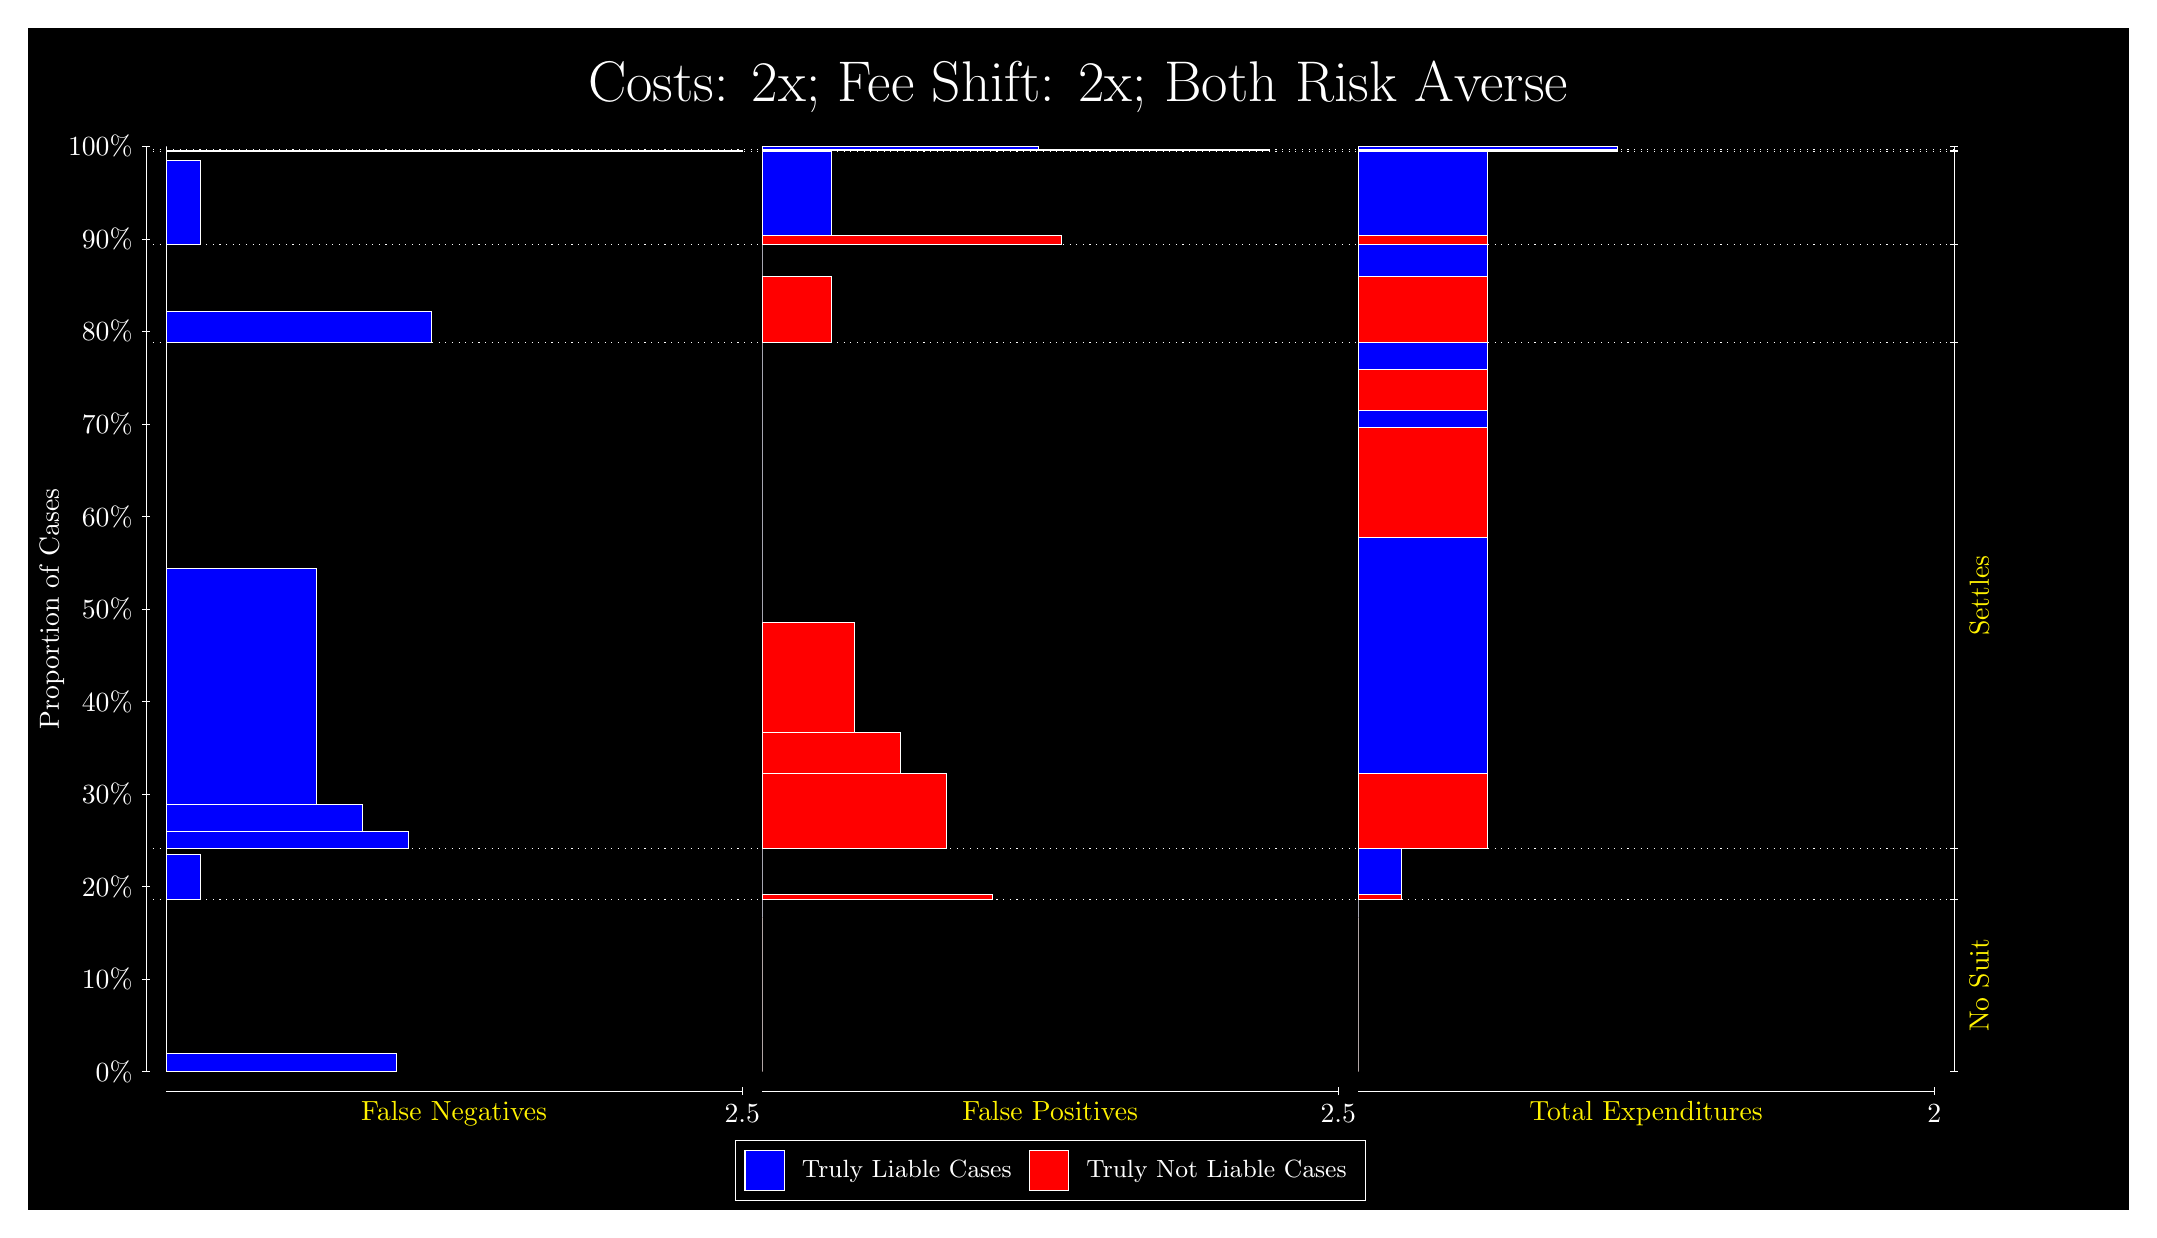
\begin{tikzpicture}
\draw[fill=black] (0,0) rectangle (26.667,15);
\draw[text=white] (0,13.5) rectangle (26.667,15) node[midway] {\huge Costs: 2x; Fee Shift: 2x; Both Risk Averse};
\draw[white, very thin] (1.5,1.75) -- (1.5,13.5);
\node[rotate=90, text=white, anchor=center] at (0.3, 7.625) {Proportion of Cases};
\draw[white, very thin] (1.45,1.75) -- (1.55,1.75);
\node[text=white, anchor=east] at (1.45, 1.75) {0\%};
\draw[white, very thin] (1.45,2.925) -- (1.55,2.925);
\node[text=white, anchor=east] at (1.45, 2.925) {10\%};
\draw[white, very thin] (1.45,4.1) -- (1.55,4.1);
\node[text=white, anchor=east] at (1.45, 4.1) {20\%};
\draw[white, very thin] (1.45,5.275) -- (1.55,5.275);
\node[text=white, anchor=east] at (1.45, 5.275) {30\%};
\draw[white, very thin] (1.45,6.45) -- (1.55,6.45);
\node[text=white, anchor=east] at (1.45, 6.45) {40\%};
\draw[white, very thin] (1.45,7.625) -- (1.55,7.625);
\node[text=white, anchor=east] at (1.45, 7.625) {50\%};
\draw[white, very thin] (1.45,8.8) -- (1.55,8.8);
\node[text=white, anchor=east] at (1.45, 8.8) {60\%};
\draw[white, very thin] (1.45,9.975) -- (1.55,9.975);
\node[text=white, anchor=east] at (1.45, 9.975) {70\%};
\draw[white, very thin] (1.45,11.15) -- (1.55,11.15);
\node[text=white, anchor=east] at (1.45, 11.15) {80\%};
\draw[white, very thin] (1.45,12.325) -- (1.55,12.325);
\node[text=white, anchor=east] at (1.45, 12.325) {90\%};
\draw[white, very thin] (1.45,13.5) -- (1.55,13.5);
\node[text=white, anchor=east] at (1.45, 13.5) {100\%};

\draw[white, very thin] (24.457,1.75) -- (24.457,13.5);
\draw[white, very thin] (24.407,1.75) -- (24.507,1.75);
\node[anchor=west] at (24.407, 1.75) {};
\draw[white, very thin] (24.407,3.9363) -- (24.507,3.9363);
\node[anchor=west] at (24.407, 3.9363) {};
\draw[white, very thin] (24.407,4.5814) -- (24.507,4.5814);
\node[anchor=west] at (24.407, 4.5814) {};
\draw[white, very thin] (24.407,11.007) -- (24.507,11.007);
\node[anchor=west] at (24.407, 11.007) {};
\draw[white, very thin] (24.407,12.256) -- (24.507,12.256);
\node[anchor=west] at (24.407, 12.256) {};
\draw[white, very thin] (24.407,13.433) -- (24.507,13.433);
\node[anchor=west] at (24.407, 13.433) {};
\draw[white, very thin] (24.407,13.456) -- (24.507,13.456);
\node[anchor=west] at (24.407, 13.456) {};
\draw[white, very thin] (24.407,13.5) -- (24.507,13.5);
\node[anchor=west] at (24.407, 13.5) {};

\draw[white, very thin, fill=blue] (1.75,1.75) rectangle (4.6775,1.98);
\draw[white, very thin, fill=red] (1.75,1.98) rectangle (1.75,3.9363);
\draw[white, very thin, fill=blue] (1.75,3.9363) rectangle (2.1891,4.5154);
\draw[white, very thin, fill=red] (1.75,4.5154) rectangle (1.75,4.5814);
\draw[white, very thin, fill=blue] (1.75,4.5814) rectangle (4.8239,4.8015);
\draw[white, very thin, fill=blue] (1.75,4.8015) rectangle (4.2384,5.1397);
\draw[white, very thin, fill=blue] (1.75,5.1397) rectangle (3.6529,8.1381);
\draw[white, very thin, fill=red] (1.75,8.1381) rectangle (1.75,11.007);
\draw[white, very thin, fill=blue] (1.75,11.007) rectangle (5.1167,11.41);
\draw[white, very thin, fill=red] (1.75,11.41) rectangle (1.75,12.256);
\draw[white, very thin, fill=blue] (1.75,12.256) rectangle (2.1891,13.317);
\draw[white, very thin, fill=red] (1.75,13.317) rectangle (1.75,13.433);
\draw[white, very thin, fill=blue] (1.75,13.433) rectangle (9.0689,13.444);
\draw[white, very thin, fill=red] (1.75,13.444) rectangle (1.75,13.456);
\draw[white, very thin, fill=red] (1.75,13.456) rectangle (1.75,13.467);
\draw[white, very thin, fill=blue] (1.75,13.467) rectangle (1.75,13.5);
\draw[white, very thin, fill=red] (9.3189,1.75) rectangle (9.3189,3.7063);
\draw[white, very thin, fill=blue] (9.3189,3.7063) rectangle (9.3189,3.9363);
\draw[white, very thin, fill=red] (9.3189,3.9363) rectangle (12.246,4.0023);
\draw[white, very thin, fill=blue] (9.3189,4.0023) rectangle (9.3189,4.5814);
\draw[white, very thin, fill=red] (9.3189,4.5814) rectangle (11.661,5.5381);
\draw[white, very thin, fill=red] (9.3189,5.5381) rectangle (11.075,6.0588);
\draw[white, very thin, fill=red] (9.3189,6.0588) rectangle (10.49,7.4499);
\draw[white, very thin, fill=blue] (9.3189,7.4499) rectangle (9.3189,11.007);
\draw[white, very thin, fill=red] (9.3189,11.007) rectangle (10.197,11.852);
\draw[white, very thin, fill=blue] (9.3189,11.852) rectangle (9.3189,12.256);
\draw[white, very thin, fill=red] (9.3189,12.256) rectangle (13.125,12.372);
\draw[white, very thin, fill=blue] (9.3189,12.372) rectangle (10.197,13.433);
\draw[white, very thin, fill=red] (9.3189,13.433) rectangle (9.3189,13.445);
\draw[white, very thin, fill=blue] (9.3189,13.445) rectangle (9.3189,13.456);
\draw[white, very thin, fill=red] (9.3189,13.456) rectangle (15.759,13.467);
\draw[white, very thin, fill=blue] (9.3189,13.467) rectangle (12.832,13.5);
\draw[white, very thin, fill=red] (16.888,1.75) rectangle (16.888,3.7063);
\draw[white, very thin, fill=blue] (16.888,3.7063) rectangle (16.888,3.9363);
\draw[white, very thin, fill=red] (16.888,3.9363) rectangle (17.437,4.0023);
\draw[white, very thin, fill=blue] (16.888,4.0023) rectangle (17.437,4.5814);
\draw[white, very thin, fill=red] (16.888,4.5814) rectangle (18.534,5.5381);
\draw[white, very thin, fill=blue] (16.888,5.5381) rectangle (18.534,8.5365);
\draw[white, very thin, fill=red] (16.888,8.5365) rectangle (18.534,9.9276);
\draw[white, very thin, fill=blue] (16.888,9.9276) rectangle (18.534,10.148);
\draw[white, very thin, fill=red] (16.888,10.148) rectangle (18.534,10.668);
\draw[white, very thin, fill=blue] (16.888,10.668) rectangle (18.534,11.007);
\draw[white, very thin, fill=red] (16.888,11.007) rectangle (18.534,11.852);
\draw[white, very thin, fill=blue] (16.888,11.852) rectangle (18.534,12.256);
\draw[white, very thin, fill=red] (16.888,12.256) rectangle (18.534,12.372);
\draw[white, very thin, fill=blue] (16.888,12.372) rectangle (18.534,13.433);
\draw[white, very thin, fill=red] (16.888,13.433) rectangle (20.181,13.445);
\draw[white, very thin, fill=blue] (16.888,13.445) rectangle (20.181,13.456);
\draw[white, very thin, fill=red] (16.888,13.456) rectangle (20.181,13.467);
\draw[white, very thin, fill=blue] (16.888,13.467) rectangle (20.181,13.5);
\draw[white, dotted] (1.5,3.9363) -- (24.457,3.9363);
\draw[white, dotted] (1.5,4.5814) -- (24.457,4.5814);
\draw[white, dotted] (1.5,11.007) -- (24.457,11.007);
\draw[white, dotted] (1.5,12.256) -- (24.457,12.256);
\draw[white, dotted] (1.5,13.433) -- (24.457,13.433);
\draw[white, dotted] (1.5,13.456) -- (24.457,13.456);
\draw[white, very thin] (1.75,1.5) -- (9.0689,1.5);
\node[text=yellow, anchor=north] at (5.4094, 1.5) {False Negatives};
\draw[white, very thin] (9.0689,1.45) -- (9.0689,1.55);
\node[text=white, anchor=north] at (9.0689, 1.45) {2.5};

\draw[white, very thin] (9.3189,1.5) -- (16.638,1.5);
\node[text=yellow, anchor=north] at (12.978, 1.5) {False Positives};
\draw[white, very thin] (16.638,1.45) -- (16.638,1.55);
\node[text=white, anchor=north] at (16.638, 1.45) {2.5};

\draw[white, very thin] (16.888,1.5) -- (24.207,1.5);
\node[text=yellow, anchor=north] at (20.547, 1.5) {Total Expenditures};
\draw[white, very thin] (24.207,1.45) -- (24.207,1.55);
\node[text=white, anchor=north] at (24.207, 1.45) {2};

\node[text=yellow, centered, rotate=90] at (24.777, 2.8432) {No Suit};

\node[text=yellow, centered, rotate=90] at (24.777, 7.794) {Settles};





\draw (12.978300999999998,1.5) node[draw=none] (baseCoordinate) {};
\begin{scope}[align=center]
        \matrix[scale=0.5, draw=white, below=0.5cm of baseCoordinate, nodes={draw}, column sep=0.1cm]{
            \node[rectangle, draw, minimum width=0.5cm, minimum height=0.5cm, fill=blue] {}; &
            \node[draw=none, font=\small, text=white] (B) {Truly Liable Cases}; &
            \node[rectangle, draw, minimum width=0.5cm, minimum height=0.5cm, fill=red] {}; &
            \node[draw=none, font=\small, text=white] (B) {Truly Not Liable Cases}; \\
            };
\end{scope}

\end{tikzpicture}
\end{document}